\newpage
\section{Prinsipiell løsning}
\label{prinsipiellLoesning}

Et anti-aliasing filter brukes for å minske aliasing når man konverter signalet fra et analogt til digitalt signal. Nyquist raten sier at samplingsfrekvensen må være minst dobbelt så høy som den høyeste frekvensen i signalet, for å kunne rekonstruere signalet etter konvertering\cite{Nyquist}. De Ideele egenskapene til et anti aliasing filter er at amplituderesopnsen er flat i passbåndet, og at den har en bratt overgang fra passbåndet til stoppbåndet. Jo, brattere overgangen er, jo bedre er filteret. Et anti-aliasing filter realiseres derfor med et veldig agresivt lavpassfilter. Et Butterworth filter vil ha bratt nok overgang til å tilfredstille kravene til et anti-aliasing filter uten å påvirke signalet for mye i passbåndet i motsetning til et Chebyshev filter som skaper ripples i passbåndet.

\subsection{Butterworth filter}
\label{ButterworthFilter}

Et Butterworth filter er et aktivt filter som kun benytter seg av kondensatorer som frekvensavhengige komponenter. Kretstopologien er basert på Sallen-Key filteret som er vist i figur \ref{fig:SallenKey}. Sallen-Key filteret er et aktivt filter som bruker to operasjonsforsterkere, to kondensatorer og to motstander\cite{SallenKey}. Filteret kan realisere et andre ordens lavpassfilter med en Butterworth karakteristikk. Kretsen er vist i figur \ref{fig:SallenKey}. 

\begin{figure} [!h]
\centering
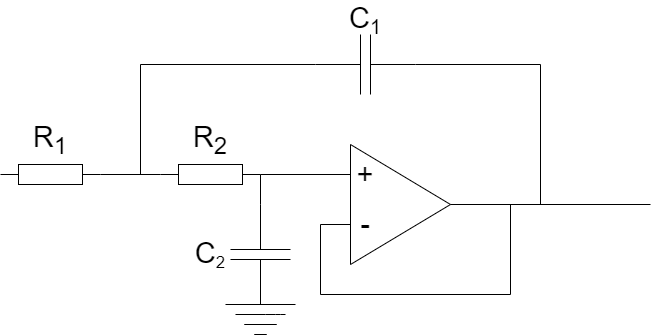
\includegraphics[width=0.7\linewidth]{Bilder/SallenKey.drawio.png}
\caption{Sallen-Key filteret}
\label{fig:SallenKey}
\end{figure}

\subsection{Finne orden av systemet}

For å finne orden til systemet kan vi bruke samme fremgangsmåte som vist av Lars Lundheim i vieoen KS3. Systemets orden kan indentefiseres ved å ta absoluttverdien av systemfunksjonen $H(j2\pi f_c)$ sammen med formelen: $A = |H(j\pi f_c)| = 10^{\frac{A[dB]}{20}}$ hvor vi gjør om systemfunksjonen fra en logaritmisk til en linær skala. For å finne den minimale orden til systemet kan man andvende formel \ref{eq:orden}. Formelen er hentet fra et designeksempel av Dr. Lundheim \cite{KS3} og benyttes for å tilfredstille kravet om -10dB dempning ved $f_B$.

\begin{equation}
\label{eq:orden}
n \geq \frac{1}{2}\frac{\ln{(A^{-2}-1)}}{+ln{(\frac{f_B}{f_c})}}
\end{equation}

Dersom vi setter inn for frekvensene gitt i dette designet får vi en orden $n \geq 3.82$ som vi runder opp til $n = 4$. Dette betyr at vi må bruke et fjerde ordens Butterworth filter for å tilfredstille kravene til filteret. For å forbedre egenskapene til filtereet så kan man benytte seg av høyere orden enn det som oppgis av formel \ref{eq:orden}. Dette vil gi et filter med en brattere overgang fra passbåndet til stoppbåndet.

\subsection{Valg av komponenter}
For å kunne implementere et n-te ordens Butterworth filter med ønske amplituderespons så er det nødvendig å vite den relative dempningsfaktoren $\zeta$ for hver indeviduelle Butterworth filter i kaskadekoblingen. En oversikt over disse verdiene er hentet fra Dr. Lundheim sin video og vises i tabell \ref{tab:zeta}

\begin{table}[!h]
    \centering
    \caption{$\zeta$-verdier for polpar, $i$, og systemorden, $n$.}
    \label{tab:zeta}
    \begin{tabular}{|c|c|c|c|c|c|}
    \hline
        & \multicolumn{5}{l|}{Polpar $i$}   \\ \hline
    $n$ & $1$       & $2$       & $3$       &      &   \\ \hline
    $1$ & 1         &           &           &      &   \\ \hline
    $2$ & $0.70711$ &           &           &      &   \\ \hline
    $3$ & 1         & $0.5$     &           &      &   \\ \hline
    $4$ & $0.92388$ & $0.38268$ &           &      &   \\ \hline
    $5$ & 1         & $0.80902$ & $0.30902$ &      &   \\ \hline
    $6$ & $0.96593$ & $0.70711$ & $0.25882$ &      &   \\ \hline
    $7$ & $1$ & $0.90097$ & $0.62349$ & $0.22252$     &   \\ \hline
    $8$ & $0.98079$ & $0.83147$ & $0.55557$ &  $0.19509$    &  \\ \hline
    $9$ & $1$ & $0.93969$ & $0.76604$ & $0.5$     &  $0.17365$ \\ \hline
    $10$ & $0.98769$ & $0.89101$ & $0.70711$ &  $0.45399$    & $0.15643$  \\ \hline
    \end{tabular}
    \end{table}

\say{Sallen-Key-byggeklossen} bruker en opamp, og da er det hensynsmessig å la 

\begin{equation}
    1\text{k}\Omega\leq R\leq100\text{k}\Omega
\end{equation}

Knekkfrekvensen gitt i radianer vil være

\begin{equation}
    w_0=2\pi f_0
\end{equation}

Hvert kondensatorpar per \say{Sallen-Key-byggekloss} vil ha egne tidskonstanter $\tau=RC$ gitt ved

\begin{equation}
    \tau_1=\frac{1}{w_0\zeta_1}, \hspace{1cm} \tau_2=\frac{1}{w_0^2\tau_1}
\end{equation}


Her er det vanelig å sette motstandene til noe mellom $1k\Omega - 100k\Omega$ for å så beregne kondensatorverdiene utifra dette. Men ettersom det finnes flere motstandsverdier og de er lettere å kombinere så kan man sette kondensatorene til noen faste verdir og så beregne motstandene utifra dette ved hjelp av linking \ref{eq:Motstander}. Dette er en mer hensynsmessig måte å gjøre det på. Normale kondensatorverdier å benytte seg av i dette tilfellet vil være $100nF, 1\mu F$ og $1.5\mu F$. For å kompensere for tilnærmingen kan man legge til et orden høyere på filteret.

\begin{equation}
    R=\frac{\tau_1}{C_1}, \hspace{1cm} R=\frac{\tau_2}{C_2}
    \label{eq:Motstander}
\end{equation}

